\documentclass{beamer}

\mode<article> % only for the article version
{
	\usepackage{fullpage}
	\usepackage{hyperref}
}

\mode<presentation>
{
	\usetheme{boxes}
	\usetheme{JuanLesPins}
}

\usepackage{astron}
\usepackage{gastex}
\usepackage{multirow}
\usepackage{algorithm}
\usepackage{algorithmic}

\usepackage{pgf,pgfarrows,pgfnodes,pgfautomata,pgfheaps,pgfshade}
\setbeamercovered{dynamic}

%Include Macro commands
%To comment out some parts for submission
\newcommand{\commM}[1]{}
\newcommand{\commE}[1]{#1}

%Frame box for formulas with minipage
\newsavebox{\ffrbox}
\newenvironment{fframe}[2] {\begin{center} \begin{lrbox}{\ffrbox} \begin{minipage}{#1\linewidth} \vspace{#2cm}}{ \end{minipage} \end{lrbox} \fbox{\usebox{\ffrbox}} \end{center}}

%Eigenvalue eigenvector
\newcommand{\vx}[1]{\overrightarrow{x_{#1}}}
\newcommand{\vxe}{\overrightarrow{x^{*}}}
\newcommand{\vxi}[1]{\overrightarrow{x\left(#1\right)}}
\newcommand{\xij}[1]{x\left(#1\right)_{j}}
\newcommand{\vxl}{\vx{\lambda}}
\newcommand{\vxli}[1]{\vx{\lambda_{#1}}}
\newcommand{\vp}{\overrightarrow{p}}

%Matric & vector norms
\newcommand{\nvec}[1]{\lVert #1 \rVert_{v} }
\newcommand{\nmat}[1]{\lVert #1 \rVert_{m} }
\newcommand{\nvece}[1]{\nvec{ #1 }^{2} }
\newcommand{\nvecinf}[1]{\nvec{ #1 }^{\infty} }
\newcommand{\nvecinfal}[1]{\nvec{ #1 }^{{\color[rgb]{0,0,1}\infty}} }
\newcommand{\nmatinf}[1]{\nmat{ #1 }^{\infty} }
\newcommand{\jinlN}[3]{#1 \in #2,..,#3} %\overline{}
\newcommand{\vInd}{\overrightarrow{i_{Ind}}}

%Complexity
\newcommand{\Oc}[1]{\mathcal{O}\left( #1 \right)} %Big o - i.e. time complexity

%Uniformization
\newcommand{\ur}{q} %uniformization rate

%CTMC & DTMC matrices
\newcommand{\mB}{\mP_{B}} %A DTMC where all bad states, i.e. not Phi and not Psi and Psi belonging to some BSCC are made absorbing
\newcommand{\mP}{\mathcal{P}} %A stochastic matrix
\newcommand{\mU}{\mP_{unif}} %Uniformized CTMC
\newcommand{\mT}{\mathcal{T}} %An irreducible submatrix of a stochastic matrix.
\newcommand{\DTMC}{\left( S,\: \mP \right)}
\newcommand{\mQ}{\mathcal{Q}} %Generator matrix
\newcommand{\mR}{\mathcal{R}} %Rate matrix
\newcommand{\CTMC}{\left( S,\: \mQ \right)}
\newcommand{\mA}{\mathcal{A}}
\newcommand{\mQnpvp}{\mQ\left[\npvp \right]}
\newcommand{\mQBnpvp}{\mQ^{B}\left[\npvp \right]}

%CTMC and transient analysis
\newcommand{\pipOti}{\pi^{*} \left(0, t \right )_{i}} %The i'th component of \vpipOt
\newcommand{\vpipOt}{\overrightarrow{\pi^{*} \left(0, t \right )}} % Transient probability, precise
\newcommand{\pipOtj}{\pi^{*} \left(0, t \right )_{j}} % The j'th component of the transient-probability vector, precise
\newcommand{\vpiOt}{\overrightarrow{\pi \left(0, t \right )}} % Transient probability, computed
\newcommand{\piOtj}{\pi \left(0, t \right )_{j}} % The j'th component of the transient-probability vector, computed


\newcommand{\pOi}{p\left( 0 \right)_{i}} % The i'th component of \vpO
\newcommand{\vpO}{\overrightarrow{p \left( 0 \right)} } % Initial distribution for a CTMC
\newcommand{\vpOi}{\overrightarrow{p(0,i)}} %The i'th iteration for uniformized DTMC, with initial distribution \vpiO
\newcommand{\pOij}{p(0,i)_{j}} %The j'th component of \vpOi
\newcommand{\vpOK}{\overrightarrow{p(0,K)}} %The K'th iteration for uniformized DTMC, with initial distribution \vpiO
\newcommand{\pOKj}{p(0,K)_{j}} %The j'th component of \vpOK
\newcommand{\vpOiM}{\overrightarrow{p(0,i+M)}} %The (i+M)'th iteration for uniformized DTMC, with initial distribution \vpiO
\newcommand{\vppO}{\overrightarrow{p^{*}(0)}} %The steady state for transient analysis, starting in state \vpiO
\newcommand{\ppOj}{p^{*}(0)_{j}} %The j'th component of \vppO
\newcommand{\ppOi}{p^{*}(0)_{i}} %The i'th component of \vppO

%CSL model checking
\newcommand{\vis}{\overrightarrow{1_{s} }} %The initial distribution for state s
\newcommand{\vpist}{\overrightarrow{\pi \left( s,t \right) }}
\newcommand{\vpit}{\overrightarrow{\pi \left( t \right) }} %The resulting probability vector for backward computations
\newcommand{\vpsi}{\overrightarrow{p(s,i)}} %An i'th iteration vector for forward computation 
\newcommand{\vpsj}[1]{\overrightarrow{p(s,#1)}} %An j'th iteration vector for forward computation 
\newcommand{\vpsim}{\overrightarrow{p(s,i{+}M)}}  %An (i+m)'th iteration vector for forward computation
\newcommand{\vpOim}{\overrightarrow{p(0,i{+}M)}}  %An (i+m)'th iteration vector for forward computation
\newcommand{\vpsK}{\overrightarrow{p(s,K)}} %A K'th iteration vector for forward computation 
\newcommand{\vpsKI}{\overrightarrow{p(s,K{+}1)}} %A K+1'th iteration vector for forward computation 
\newcommand{\vpi}{\overrightarrow{p(i)}} %An i'th iteration vector for backward computation
\newcommand{\vpK}{\overrightarrow{p(K)}} %An K'th iteration vector for backward computation
\newcommand{\vpKI}{\overrightarrow{p(K{+}1)}} %An K+1'th iteration vector for backward computation
\newcommand{\vpiM}{\overrightarrow{p(i{+}M)}} %An (i+m)'th iteration vector for backward computation
\newcommand{\vpipt}{\overrightarrow{\pi^{*} \left( t \right)}} % A precise solution of equation for backward computations
\newcommand{\vpipst}{\overrightarrow{\pi^{*} \left(s, t \right)}}  % A precise solution of equation for forward computations
\newcommand{\vpps}{\overrightarrow{p^{*}(s)}} % The precise steady-state vector for forward computation
\newcommand{\vpp}{\overrightarrow{p^{*}}} % The precise steady-state vector for backward computation
\newcommand{\vipsi}{\overrightarrow{i_{\Psi}}}
\newcommand{\vibad}{\overrightarrow{i_{\BPsi \cup \SNPhi}}}
\newcommand{\vbpi}{\overrightarrow{p^{B}\left( i \right)}}
\newcommand{\vbpK}{\overrightarrow{p^{B}\left( K \right)}}
\newcommand{\bpij}{p^{B}\left( i \right)_{j}}

\newcommand{\ipsij}{i_{\Psi,j}}  %The j'th component of \vipsi
\newcommand{\pitj}{\pi \left( t \right)_{j}}
\newcommand{\pits}{\pi \left( t \right)_{s}}
\newcommand{\piptj}{\pi^{*} \left( t \right)_{j}}
\newcommand{\pipts}{\pi^{*} \left( t \right)_{s}}
\newcommand{\pistj}{\pi \left(s, t \right)_{j}}
\newcommand{\pipstj}{\pi^{*} \left(s, t \right)_{j}}
\newcommand{\pij}{p(i)_{j}} % The j'th component of the i'th iterate for backward computation
\newcommand{\pilj}{p(i+1)_{j}} % The j'th component of the i+1'th iterate for backward computation
\newcommand{\pKj}{p(K)_{j}} % The j'th component of the K'th iterate for backward computation
\newcommand{\ppj}{p^{*}_{j}} % The j'th component of the precise steady-state vector for backward computation
\newcommand{\psij}{p(s,i)_{j}} % The j'th component of the i'th iterate for forward computation starting from state s
\newcommand{\psji}[2]{p(s,#1)_{#2}} % The i'th component of the j'th iterate for forward computation starting from state s
\newcommand{\pjik}{p(j,i)_{k}} % The k'th component of the i'th iterate for forward computation, starting from state j
\newcommand{\psiNl}{p(s,i)_{N{-}1}} % The N-1'th component of the i'th iterate for forward computation
\newcommand{\psiN}{p(s,i)_{N}} % The N'th component of the i'th iterate for forward computation
\newcommand{\psKNI}{p(s,K)_{N{-}1}} % The N-1'th component of the K'th iterate for forward computation
\newcommand{\psKINI}{p(s,K+1)_{N{-}1}} % The N-1'th component of the K+1'th iterate for forward computation
\newcommand{\psKIN}{p(s,K{+}1)_{N}} % The N'th component of the K+1'th iterate for forward computation
\newcommand{\psKN}{p(s,K)_{N}} % The N'th component of the K'th iterate for forward computation
\newcommand{\psKj}{p(s,K)_{j}} % The j'th component of the K'th iterate for forward computation
\newcommand{\psKZj}{p(s,K{+}Z)_{j}} % The j'th component of the K+Z'th iterate for forward computation

\newcommand{\psKIj}{p(s,K{+}1)_{j}} % The j'th component of the K+1'th iterate for forward computation
\newcommand{\ppsj}{p^{*}(s)_{j}} % The j'th component of the precise steady-state vector for forward computation
\newcommand{\ppsNl}{p^{*}(s)_{N{-}1}} % The N-1'th component of the precise steady-state vector for forward computation
\newcommand{\ppsN}{p^{*}(s)_{N}} % The N'th component of the precise steady-state vector for forward computation

%For the stopping criteria
\newcommand{\psjk}[1]{p\left(s,#1\right)_{k}}
\newcommand{\tmaxk}{t_{k}^{max}}  %the max probability to go from a transient state to and absorbing state k in one step

%Poisson 
\newcommand{\pnd}{e^{-\ur t}\frac{\left( \ur t \right)^{i}}{i!}}
\newcommand{\gpqt}[1]{\gamma_{#1}(t)}
\newcommand{\giqt}{\gpqt{i}}
\newcommand{\gjqt}{\gpqt{j}}

%Fox-Glynn
\newcommand{\ltp}{\mathcal{L}_{\epsilon}} %Left truncation point
\newcommand{\rtp}{\mathcal{R}_{\epsilon}} %Right truncation point
\newcommand{\wi}{w_{i}(t)} %The i'th weight

%Misc
\newcommand{\ToDo}[1]{ 
                                          \begin{center} 
                                          *************************** ToDo ***************************\\
                                          \emph{#1}\\
                                          ************************************************************
                                          \end{center} 
                                        }
\newcommand{\eqnapp}[1]{
                                            \renewcommand{\theequation}{#1.\arabic{equation}}
                                            % redefine the command that creates the equation no.
                                            \setcounter{equation}{0}  % reset counter 
                                          }

%Good and Bad states
	%Sets of states
	\newcommand{\Ind}{Ind} %A set of indexes
	\newcommand{\Gl}{\mathcal{G}} %Goal states
	\newcommand{\Al}{\mathcal{A}} %Allowed states
	\newcommand{\Il}{\mathcal{I}} %Illegal states those which are no \Al and not \Gl
	\newcommand{\Bag}{B_{ \Al, \Gl }} %The bad states to make absorbing
	\newcommand{\vigl}{\overrightarrow{1_{\Gl}}}
	\newcommand{\viind}{\overrightarrow{1_{\Ind}}}
	\newcommand{\AlMBagGl}{\Al \setminus \left( \Gl \cup \Bag \right)}

	%Matrices
	\newcommand{\mQnavg}{\mQ\left[ \Il \cup \Gl \right]}

	%Probabilistic Time reachability
	\newcommand{\PZsf}[3]{\mathrm{P}_{#1}(#2, \:#3)}
	\newcommand{\ppUp}[4]{#1 \: \mathrm{U}^{[#2,#3]} \: #4}
	\newcommand{\PZsaUg}[4]{\PZsf{#1}{#2}{\ppUp{\Al}{#3}{#4}{\Gl}}}
	
	\newcommand{\PZaUg}[3]{\PZf{#1}{\ppUp{\Al}{#2}{#3}{\Gl}}}

	\newcommand{\Psf}[2]{\mbox{\it Prob}(#1, \: #2 )}
	\newcommand{\Pf}[1]{\mathrm{P}( #1 )}
	\newcommand{\PsaUg}[3]{\Psf{#1}{\ppUp{\Al}{#2}{#3}{\Gl}}}
	\newcommand{\PsSUg}[3]{\Psf{#1}{\ppUp{S}{#2}{#3}{\Gl}}}
	
	%Vectors
	\newcommand{\vibadag}{\overrightarrow {i_{\Bag \cup \Il}}}

%PRCTL
\newcommand{\Y}[2]{{\cal Y}^{#1}_{#2}}
\newcommand{\Prob}[3]{{\cal P}_{#1 #2}(#3)}

%CSL
	%Steady-state operator
	 \newcommand{\SpsP}[3]{\mathrm{S}_{\trianglelefteq #1}(#2,\: #3)}
	 
	 %Next operator
	 \newcommand{\Xp}[3]{\mathrm{X}^{[#1,\:#2]} \: #3}
	 
	%Until operator
	\newcommand{\ttUp}[2]{\ppUp{tt}{#1}{#2}{\Psi}}  %The time bounded true Until Psi formula
	\newcommand{\pUp}[2]{\ppUp{\Phi}{#1}{#2}{\Psi}}  %The time bounded Phi Until Psi formula
	
	%Bounded probability and until operator with some initial state
	\newcommand{\PZf}[2]{\mathrm{P}_{#1}(#2)}
	\newcommand{\PZspUp}[4]{\PZsf{#1}{#2}{\pUp{#3}{#4}}}
	\newcommand{\PZsttUp}[4]{\PZsf{#1}{#2}{\ttUp{#3}{#4}}}
	\newcommand{\PZpUp}[3]{\PZf{#1}{\pUp{#2}{#3}}}

	%Probability for state formula with some initial state
	\newcommand{\PspUp}[3]{\Psf{#1}{\pUp{#2}{#3}}}
	\newcommand{\PsttUp}[3]{\Psf{#1}{\ttUp{#2}{#3}}}
	
	%Some bad states, we make absorbing
	\newcommand{\BPsi}{\mathrm{B}_{\Psi}}

%CSRL
	%Until reward operator
	\newcommand{\ppUrp}[6]{#1 \: \mathrm{U}^{{\tiny [#2,#3]}}_{{\tiny [#4,#5]}} \: #6}
	\newcommand{\pUrp}[4]{\ppUrp{\Phi}{#1}{#2}{#3}{#4}{\Psi}}  %The time bounded Phi Until Psi formula

	\newcommand{\npvp}{\lnot \Phi \vee \Psi}
	\newcommand{\Sat}[1]{Sat \left(#1 \right)} % The set of states satisfying \Psi
	\newcommand{\SPsi}{\Sat{\Psi}} % The set of states satisfying \Psi
	\newcommand{\SPhi}{\Sat{\Phi}} % The set of states satisfying \Psi
	\newcommand{\SNPhi}{\Sat{\lnot \Phi}} % The set of states satisfying \not \Psi
	\newcommand{\Bpp}{B_{ \Phi, \Psi }} %The bad states to make absorbing
	\newcommand{\mQB}{\mQ^{B}} %The \mQ[\npvp] matrix with \Bpp states made absorbing

%Tools
	\newcommand{\prism}{\emph{Prism v2.1}}
	\newcommand{\etmcc}{\emph{ETMCC v1.4.2}}
	\newcommand{\mrmc}{\emph{MRMC v1.0}}
	\newcommand{\ultrasan}{\emph{UltraSAN v3.0}}


\title{Safe On-The-Fly Steady-State Detection for Time-Bounded Reachability}
\author[Katoen, Zapreev]{
	Joost-Pieter Katoen\inst{1,2} \and
	Ivan S. Zapreev\inst{1,2}
}
\institute[Universities of Twente and Aachen]{
  \inst{1}%
  Software Modeling and Verification Group\\
  RWTH Aachen
  \and
  \inst{2}%
  Formal Methods and Tools Group\\
  University of Twente}

\begin{document}

\bibliographystyle{astron}

\frame{\titlepage}

\section[Outline]{}
\frame{\tableofcontents}

\section{Introduction}	

\frame{
       \frametitle{Outline}
       \tableofcontents[currentsection]
}

\frame{
	\frametitle{Motivation}

	\begin{block}{The time-bounded reachability problem for continuous-time Markov chains}
		\begin{enumerate}
			\item Determine the probability to reach a (set of) goal state(s) within a given time span, such that prior to reaching the goal certain states are avoided.
			\item Efficient algorithms for time-bounded reachability are at the heart of probabilistic model checkers such as PRISM and ETMCC.
			\item For large time spans, on-the-fly steady-state detection is commonly applied.
			\item To obtain correct results (up to a given accuracy), it is essential to avoid detecting premature stationarity.
		\end{enumerate}
	\end{block}
}

\frame
{
	\frametitle{DTMC \& CTMC}
	\begin{definition}
		A Discrete-time Markov Chain (\emph{DTMC}) $\DTMC$
		\begin{itemize}
			\item $S$ - a finite set of states
			\item $\mP$ - a \emph{stochastic} matrix, $\mP \: : \: S \times S \rightarrow \left[0,\:1 \right]$, $\mP=\left(p_{i,j}\right)$
				{\small
				\begin{itemize}
					\item $\forall i \in S \: : \: \sum_{j=1}^{|S|} p_{i,j}=1$
				\end{itemize}
				}
		\end{itemize}
	\end{definition}
	\begin{definition}
		A Continuous-time Markov Chain (\emph{CTMC}) $\CTMC$
		\begin{itemize}
			\item $S$ - a finite set of states
			\item $\mQ$ - a \emph{generator} matrix, $\mQ \: : \: S \times S \rightarrow \mathbb{R}_{\geq 0}$, $\mQ=\left(q_{i,j}\right)$
				{\small
				\begin{itemize}
					\item $\mQ=\left(q_{i,j}\right)$ and $\forall i \in S \: : \: q_{i,i} = -\sum_{j, \: i \neq j} q_{i,j}$
					\item $\forall i \neq j$, $q_{i,j}$ the rate of going from $i$ to $j$.
				\end{itemize}
				}
		\end{itemize}
	\end{definition}
}

\frame
{
	\frametitle{Stationary probabilities, DTMC \cite{Haverkort_98}}
	\begin{definition}
		For a DTMC $\DTMC$ the \emph{limiting} distribution
		\begin{equation}
			\vppO = lim_{n \to \infty} \: \vpO \cdot \mP^{n}
			\label{eq:ssl_dtmc}
		\end{equation}
		where $\vpO$ is the initial distribution.
	\end{definition}
	\begin{theorem}
		For an \alert{aperiodic} DTMC $\DTMC$ and an initial distribution $\vpO$, the \emph{limiting} distribution (\ref{eq:ssl_dtmc}) exists.
	\end{theorem}
}

\frame
{
	\frametitle{Power Iterations  \cite{Stewart_94}}
	{\small
		\begin{definition}
			For a \emph{stochastic} matrix $\mP$ and an initial vector $\vxi{0}$:
			\begin{equation}
				\vxi{m} = \vxi{m{-}1}{\cdot}\mP \nonumber
			\end{equation}
		\end{definition}
		\begin{theorem}
			For an \alert{aperiodic} $\mP$ there exists $\vxe = lim_{m \to \infty} \: \vxi{m}$ equal to the \emph{dominant eigenvector} of $\mP$.
		\end{theorem}
		\begin{lemma}
			For a stochastic matrix $\mP$, the number $K$ such that $\vxi{K}$ is $\epsilon$-close to $\vxe$ may be approximated by:
			\begin{equation}
				K = \dfrac{\log \epsilon}{log | \lambda_{2} |}, \: \lambda_{2} \textrm{ - subd. e.v. of }\mP \nonumber
			\end{equation}
		\end{lemma}
	}
}
	
\frame
{
	\frametitle{Convergence \cite{Stewart_94}}
	
	\begin{block}{Tests for convergence}
		For some $M>0$ there are the following \emph{convergence tests}:
		\begin{itemize}
			\item Absolute: $\nvec{\vxi{i} - \vxi{i{+}M}} < \varepsilon$
			\item Relative: $\max_{\jinlN{j}{1}{N}} \left( \frac{ | \xij{i{+}M} - \xij{i} |}{ | \xij{i{+}M} |} \right) < \varepsilon$
			\item etc ...
		\end{itemize}
	\end{block}
	
	\begin{alertblock}{Warning!}
		\emph{None of these convergence tests is precise.}
	\end{alertblock}
}

\section{Transient analysis}

\frame{
       \frametitle{Outline}
       \tableofcontents[currentsection]
}

\frame
{
	\frametitle{Transient analysis}
	\begin{block}{Transient probabilities of a CTMC}
		For a CTMC $\CTMC$ the state-probability after a delay of $t$ time-units
		\begin{equation}
			\vpipOt = \vpO \cdot e^{\mQ{\cdot}t}
			\nonumber
		\end{equation}
		where $\vpO$ is the initial distribution.
	\end{block}
	
	\begin{definition}
		For a CTMC $\CTMC$ an uniformized DTMC $\mP$ is
		\[
			\mP=\frac{\mQ}{\ur}+\mathcal{I}
		\]
		where $\ur \geq \max_{i \in S}| q_{i,i} |$ and $\mathcal{I}$ is the identity matrix.
	\end{definition}
}

\frame{
       \frametitle{Transient analysis}

	{\small
       \begin{block}{Jensen's method (Uniformization)}
		\begin{itemize}
			\item Substitute $\mQ$ with $\mP$:
				\begin{center}
					$\vpipOt = e^{-qt} \cdot \vpO \cdot e^{\mP \cdot qt}$
				\end{center}
			\item Use the matrix exponent definition:
				\vspace{-0.3cm}
				\begin{equation}
					\vpipOt = \sum_{i=0}^{\infty}\giqt {\cdot} \vpOi
					\label{eq:until_general}
				\end{equation}
				\vspace{-0.6cm}
		\end{itemize}
		\begin{description}
			\item[$\giqt$] $=\pnd$ - \emph{Poisson} density function
			\item[$\vpOi$] $=\vpO {\cdot} \mP^{i}$
		\end{description}
	\end{block}
	
	\begin{block}{Notice!}
		Taking  $\ur \alert{>} \max_{i \in S} |q_{i,i}|$ makes DTMC $\DTMC$ \alert{aperiodic}
	\end{block}
	}
}

\section{The Fox-Glynn algorithm}

\frame{
       \frametitle{Outline}
       \tableofcontents[currentsection]
}

\frame<1>[label=foxglynn]{
       \frametitle{The Fox-Glynn algorithm \cite{FoxG_ACM88}}

	\only<1>{
		\begin{lemma}
			For real-valued function $f$ with $\|f\| = \sup_{i \in \mathbb{N}}|f(i)|$ and $\sum_{i=\ltp}^{\rtp} \giqt \geq 1 - \frac{\varepsilon}{2}$ it holds:
				{\small
				\[
					\left| {\color[rgb]{0,0,1}\sum_{i=0}^{\infty} \giqt f(i)} - \frac{1}{W}\sum_{i = \ltp}^{\rtp} \wi f(i) \right| \leq \varepsilon \cdot \|f\| \quad
				\]
				}
		\end{lemma}
		\begin{minipage}{0.5\linewidth}
			\begin{block}{Where}
				${\color[rgb]{0,0,1} \giqt} = \pnd $\\
				${\color[rgb]{0,0,1} \alpha} \neq 0$, some constant\\
				${\color[rgb]{0,0,1} \wi} = \alpha \giqt$\\
				${\color[rgb]{0,0,1} W} = w(\ltp)+ \ldots + w(\rtp)$
			\end{block}
		\end{minipage} \hfill
		\begin{minipage}{0.45\linewidth}
			\begin{center}
				%see: ../../../../Internal Documents/Steady State Detection/poisson.eps
				\hyperlink{foxglynn<2>}{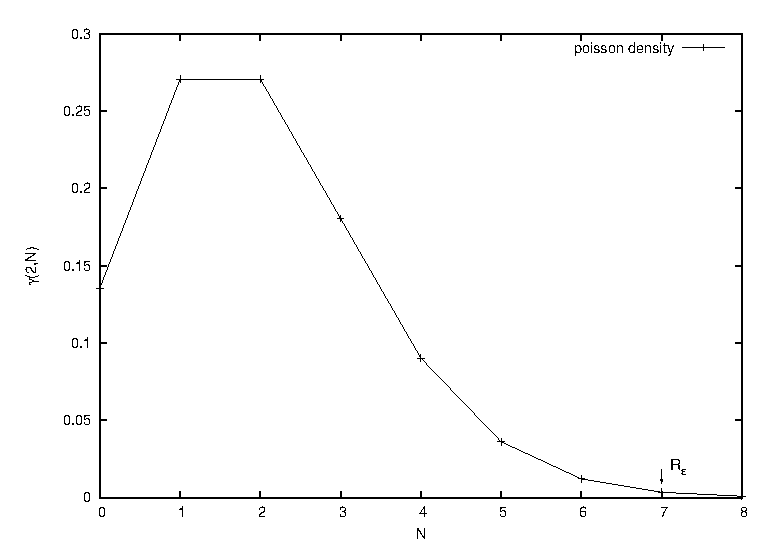
\includegraphics[scale=0.35, angle=0]{poisson.eps}}
			\end{center}
		\end{minipage}
	}
	
	\only<2>{
		\begin{center}
			%see: ../../../../Internal Documents/Steady State Detection/poisson.eps
			\hyperlink{foxglynn<1>}{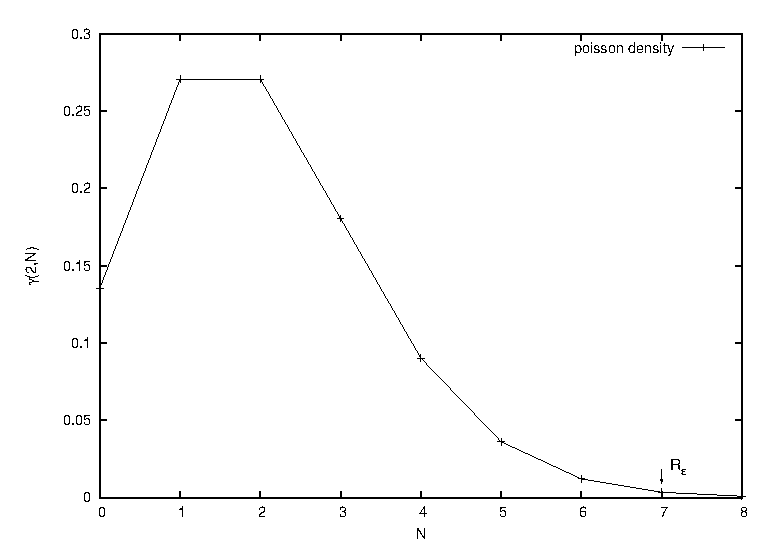
\includegraphics[scale=0.8, angle=0]{poisson.eps}} 
		\end{center}
	}
}

\frame {
	\frametitle{The Fox-Glynn algorithm - refinement}

	\begin{block}{Errors}
		\begin{itemize}
			\item $\ltp$ and $\rtp$, each, give error $\frac{\epsilon}{4}$
			\item Normalization $\frac{\wi}{W}$gives additional $\frac{\epsilon}{2}$
		\end{itemize}
	\end{block}

	\begin{alertblock}{Lemma}
		For real-valued function {\color[rgb]{0,0,1} $f$ that does not change sign} with $\|f\| = \sup_{i \in \mathbb{N}}|f(i)|$ and $\sum_{i=\ltp}^{\rtp} \giqt \geq 1 - \frac{\varepsilon}{2}$ it holds:
		{\small
			\begin{equation}
				\left| \sum_{i=0}^{\infty} \giqt f(i) - \frac{1}{W}\sum_{i = \ltp}^{\rtp} \wi f(i) \right| \leq {\color[rgb]{0,0,1} \frac{\varepsilon}{2} } \cdot \|f\| \quad
				\label{pr:fg_imp}
			\end{equation}
		}
	\end{alertblock}
}

\section{Transient probabilities and the steady-state}

\frame{
       \frametitle{Outline}
       \tableofcontents[currentsection]
}

\frame{
	\frametitle{Limiting distribution and transient probabilities}
	\begin{block}{Steady-state detection \cite{ReibmanT_COR88}}
		For the case of an \alert{aperiodic} DTMC $\DTMC$, the Power iteration in (\ref{eq:until_general}) converges:
		\[
			\vppO = lim_{i \to \infty} \: \vpOi = lim_{i \to \infty} \vpO {\cdot} \mP^{i}
		\]
		Then in 
		\[
			\vpipOt = \sum_{i=0}^{\infty}\giqt {\cdot} \vpOi
		\]
		starting from some $i$ the $\vppO$ can be used instead of $\vpOi$.
	\end{block}
}

\frame{
	\frametitle{Computing transient probabilities \cite{MalhotraMT_MR94} }
	\begin{alertblock}{Computations with Steady-state detection}
	\small{
		Let $\exists K : \forall i \geq K : \nvec{\vppO - \vpOi} \leq \delta$.
			\begin{equation}
			\displaystyle
			\vpiOt = \left\{
			\begin{array}{ll}
				\vpOK & \text{, if } K < \ltp\\
				\sum_{i=\ltp}^{K}\giqt \vpOi + & \\
				\vpOK \left(1- \sum_{i=0}^{K}\giqt \right) & \text{, if } \ltp \leq K \leq \rtp\\
				\sum_{i=\ltp}^{\rtp}\giqt \vpOi & \text{, if } K > \rtp\\
			\end{array}
			\right .
			\label{eq:ssd_LR}
		\end{equation}
		Then if $\sum_{i=0}^{\ltp} \giqt \leq \frac{\epsilon}{2}$ and $\sum_{i=\rtp}^{\infty} \giqt \leq \frac{\epsilon}{2}$: 
		\begin{fframe}{0.6}{-0.0}
			\[
				\nvec{\vpipOt - \vpiOt} \ \leq \ 2 \delta + \frac{\varepsilon}{2}
			\]
		\end{fframe}
	}
	\end{alertblock}
}

\frame{
	\frametitle{Criteria}

	\begin{block}{A corollary}
		\begin{fframe}{0.68}{-0.2}
			\begin{eqnarray}
				\nvec{\vppO - \vpOK} \leq \frac{\varepsilon}{4} \nonumber \text{ implies } \\
				\nvec{\vpipOt - \vpiOt} \leq \varepsilon
				\nonumber
			\end{eqnarray}
		\end{fframe}
	\end{block}
		
	\begin{alertblock}{The actual steady-state detection criteria}
		\begin{itemize}
			\item Take $K = i + M$ if 
				\[
					\nvec{{\color[rgb]{0,0,1} \vpOi} - \vpOiM} \leq \frac{\varepsilon}{4} \quad \mbox{for } M > 0
				\]
			\item Check this condition every $M$ iterations
		\end{itemize}
	\end{alertblock}
}

\frame{
	\frametitle{The known problems}
	
	\begin{alertblock}{Problems}
		\begin{enumerate}
			\item \emph{The steady-state detection is uncertain} - due to the criteria
			\item \emph{The error bound is not precise} - as derived under an assumption of knowing \emph{real} steady-state. \label{it:p2}
			\item \emph{The norm $\nvec{.}$ is not defined} - was assumed that:
				\begin{equation}
					\nvec{\vpOi} \leq 1 \nonumber
				\end{equation}
			\item \emph{The weights are not considered} - if the complete Fox-Glynn algorithm is used. \label{it:p4}
		\end{enumerate}
	\end{alertblock}
}

\section{Time-bounded reachability}

\frame{
       \frametitle{Outline}
       \tableofcontents[currentsection]
}

\frame{
	\frametitle{Time-bounded reachability}
	\begin{example}
		Determine states from which goal states may be reached with a probability at least $0.92$, within the time interval $[0,14.5]$, while visiting only allowed states.
		\[
			\PZaUg{\geq 0.92}{0}{14.5}
		\]
		\begin{description}
			\item[$\Al$] - allowed states
			\item[$\Gl$] - goal states
		\end{description}
	\end{example}
	\begin{definition}
		For CTMC $\CTMC$ and $S' \subseteq S$ let CTMC $(S, \mQ')$  be obtained by making all states in $S'$ absorbing, i.e., $\mQ' = \mQ[S']$ where $q'_{i,j} = q_{i,j}$ if $i \not\in S'$ and 0 otherwise.
	\end{definition}
}

\frame{
	\frametitle{Computing $\PsaUg{s}{0}{t}$}
	\begin{block}{Forward algorithm}
		\begin{itemize}
			\item Determine $\mQnavg$
			\item Compute $\alert{\vpipst} = {\color[rgb]{0,0,1} \vis} \cdot e^{\mQnavg t}$
			\item Return $\PsaUg{s}{0}{t} = {\color[rgb]{0,0,1}\sum_{j \in \Gl}\pipstj}$
		\end{itemize}
	\end{block}
	\begin{block}{Backward algorithm}
		\begin{itemize}
			\item Determine $\mQnavg$
			\item Compute $\alert{\vpipt} = e^{\mQnavg t} \cdot {\color[rgb]{0,0,1}\vigl}$
			\item Return $\forall \jinlN{s}{1}{N} : \PsaUg{s}{0}{t} = {\color[rgb]{0,0,1} \pipts}$
		\end{itemize}
	\end{block}
}

\frame{
	\frametitle{Backward computations, algorithm \cite{YounesKNP_TACAS04}}
	\begin{alertblock}{Computations with Steady-state detection}
	\small{
		Let $\exists K : \forall i \geq K:\nvec{\vpp - \vpi} \leq \delta$.
		\begin{equation}
			\displaystyle
			\vpit = \left\{
			\begin{array}{ll}
				\vpK & \text{, if } K < \ltp\\
				\sum_{i=\ltp}^{K}\giqt \vpi + & \\ \vpK \left(1- \sum_{i= {\color[rgb]{0,0,1} \ltp}}^{K}\giqt \right) & \text{, if } \ltp \leq K \leq \rtp\\
				\sum_{i=\ltp}^{\rtp}\giqt \vpi & \text{, if } K > \rtp\\
			\end{array}
			\right .
			\label{eq:ssd_LR_b}
		\end{equation}
		Then if $\sum_{i=0}^{\ltp} \giqt \leq \frac{\epsilon}{2}$ and $\sum_{i=\rtp}^{\infty} \giqt \leq \frac{\epsilon}{2}$: 
		\begin{fframe}{0.5}{-0.0}
			\[
				\nvec{ \vpipt - \vpit } \leq 2 \delta + \frac{\varepsilon}{2}
			\]
		\end{fframe}
	}
	\end{alertblock}
}

\frame[label=regular]{
	\frametitle{Criteria}

	\begin{block}{A corollary}
		\begin{fframe}{0.78}{-0.2}
			\begin{eqnarray}
				\nvec{\vpp - \vpK} \leq {\color[rgb]{0,0,1} \frac{\varepsilon}{8}} \text{ implies } \nonumber \\
				\forall j \in S : -\frac{\varepsilon}{4} \leq \piptj - \pitj \leq \frac{3}{4}\varepsilon \nonumber
			\end{eqnarray}
		\end{fframe}
	\end{block}
		
	\begin{block}{The actual steady-state detection criteria}
		\begin{itemize}
			\item Take $K = i + M$ if 
				\[
					\nvec{{\color[rgb]{0,0,1} \vpi} - \vpK} \leq {\color[rgb]{0,0,1} \frac{\epsilon}{8}}
				\]
			\item Check this condition every $M$ iterations
		\end{itemize}
	\end{block}
}

\frame{
	\frametitle{The known problems}
	
	\begin{alertblock}{Problems}
		\begin{enumerate}
			\item \emph{The error bound for (\ref{eq:ssd_LR_b}) can be refined} - $\forall \jinlN{j}{1}{N}, \forall \jinlN{i}{0}{\infty} \: : \: \pij \leq \pilj $. \label{it:p5}
			\item \emph{An additional error is introduced} -  while switching from (\ref{eq:ssd_LR}) to (\ref{eq:ssd_LR_b}), $i=0$ became $i=\ltp$. \label{it:p6}
			\item \emph{The refinement, done in \cite{YounesKNP_TACAS04}, for (\ref{eq:ssd_LR}) and (\ref{eq:ssd_LR_b}) is incorrect} - the length of the error interval does not matter. \label{it:p7} 
		\end{enumerate}
	\end{alertblock}
}
\section{Steady-state detection, error-bound refinement}

\frame{
       \frametitle{Outline}
       \tableofcontents[currentsection]
}

\frame{
	\frametitle{Choosing the "right" norm}
	\begin{block}{Facts}
		\begin{itemize}
			\item The error estimate is based on \emph{G}eometrical \emph{C}onvergence
			\item \emph{G.C.} is proved, using \emph{total variation norm} which, in an {$N$-dimensional space}, $\nvecinf{v} = \max_{\jinlN{i}{1}{N}} |v_{i}|$.
			\item In a finite dimensional space all norms are equivalent.
		\end{itemize}
	\end{block}
	
	\begin{alertblock}{Caution!}
		The $\vigl$ vector is not a distribution, $\forall \jinlN{j}{1}{N}\: : \: 0 \leq \pij \leq 1$.
	\end{alertblock}
	
	\begin{example}
		For $N$ states and Euclidean Norm $\nvece{.}$: \\
		$\:\:\:\:\:\:\:\:\nvece{\sum_{i=0}^{\ltp-1} \giqt \vpi} \nleq \frac{\epsilon}{4}$ {\color[rgb]{1,0,0} BUT}
		$\nvece{\sum_{i=0}^{\ltp-1} \giqt \vpi} \leq \frac{\sqrt{N}}{4}\epsilon$
	\end{example}
}

\frame{
	\frametitle{Refined steady-state detection error}
	\begin{alertblock}{Forward Computations}
	\small{
		Let $\exists K :\forall i \geq K : \nvecinfal{\vppO - \vpOi} \leq \delta$.
		\begin{equation}
			\displaystyle
			\vpiOt = \left\{
			\begin{array}{ll}
				\vpOK & \text{, if } K < \ltp\\
				{\color[rgb]{0,0,1}\frac{1}{W}} \sum_{i=\ltp}^{K}{\color[rgb]{0,0,1}\wi} \vpOi + & \\
				\vpOK \left(1- {\color[rgb]{0,0,1}\frac{1}{W}} \sum_{i={\color[rgb]{0,0,1}\ltp}}^{K}{\color[rgb]{0,0,1}\wi} \right) & \text{, if } \ltp \leq K \leq \rtp\\
				{\color[rgb]{0,0,1}\frac{1}{W}} \sum_{i=\ltp}^{\rtp}{\color[rgb]{0,0,1}\wi} \vpOi & \text{, if } K > \rtp\\
			\end{array}
			\right .
			\nonumber
		\end{equation}
		Then if $\sum_{i=0}^{\ltp} \giqt \leq {\color[rgb]{0,0,1}\frac{\epsilon}{4}}$, $\sum_{i=\rtp}^{\infty} \giqt \leq {\color[rgb]{0,0,1}\frac{\epsilon}{4}}$:
		\begin{fframe}{0.85}{-0.0}
			\[
				\left| {\color[rgb]{0,0,1}\sum_{j \in \Ind}} \left( \pipOtj - \piOtj \right) \right| \leq 2 \delta {\color[rgb]{0,0,1}|\Ind|} + {\color[rgb]{0,0,1}\frac{3}{4}} \varepsilon
			\]
		\end{fframe}
	}
	\end{alertblock}
}

\frame{
	\frametitle{Refined steady-state detection error}
	\begin{alertblock}{Backward Computations}
	\small{
		Let $\exists K : \forall i \geq K : \forall \jinlN{j}{1}{N} : 0 \leq \ppj - \pij \leq \delta$.
		\begin{equation}
			\displaystyle
			\vpit = \left\{
			\begin{array}{ll}
				\vpK & \text{, if } K < \ltp\\
				{\color[rgb]{0,0,1}\frac{1}{W}} \sum_{i=\ltp}^{K} {\color[rgb]{0,0,1}\wi} \vpi + & \\
				\vpK \left(1- {\color[rgb]{0,0,1}\frac{1}{W}} \sum_{i=\ltp}^{K} {\color[rgb]{0,0,1}\wi} \right) & \text{, if } \ltp \leq K \leq \rtp\\
				{\color[rgb]{0,0,1}\frac{1}{W}} \sum_{i=\ltp}^{\rtp} {\color[rgb]{0,0,1}\wi} \vpi & \text{, if } K > \rtp\\
			\end{array}
			\right .
			\nonumber
		\end{equation}
		Then if $\sum_{i=0}^{\ltp} \giqt \leq {\color[rgb]{0,0,1}\frac{\epsilon}{4}}$, $\sum_{i=\rtp}^{\infty} \giqt \leq {\color[rgb]{0,0,1}\frac{\epsilon}{4}}$:
		\begin{fframe}{0.5}{-0.0}
			\[
				\nvecinfal{ \vpipt - \vpit } \leq {\color[rgb]{0,0,1}\delta} + {\color[rgb]{0,0,1}\frac{3}{4}} \varepsilon
			\]
		\end{fframe}
	}
	\end{alertblock}
}

\frame{
	\frametitle{Steady-state detection criteria}

	\begin{alertblock}{Forward}
		\begin{enumerate}
			\item Steady-state is detected if $\nvecinfal{{\color[rgb]{0,0,1}\vppO} - \vpOK} \leq \frac{\varepsilon}{8 |\Ind|}$
			\item Use the Fox-Glynn algorithm with desired error $\frac{\epsilon}{2}$
			\item Then the overall error bound for the computed probability $\PsaUg{s}{0}{t}$ will be $\epsilon$
		\end{enumerate}
	\end{alertblock}

	\begin{alertblock}{Backward}
		\begin{enumerate}
			\item Steady-state is detected if $\nvecinfal{{\color[rgb]{0,0,1}\vpp} - \vpK} \leq \frac{\varepsilon}{4}$
			\item Use the Fox-Glynn algorithm with desired error $\frac{\epsilon}{2}$
			\item Then the overall error bound for computed probability $\PsaUg{s}{0}{t}$, will be $\epsilon$
		\end{enumerate}
	\end{alertblock}
}

\frame{
	\frametitle{Comparing the results}
	%{\small
		\begin{table}
			\begin{center}
				\begin{tabular}{|c|c|}
					\hline
					\multicolumn{2}{|c|}{Forward} \\
					\hline
					\multicolumn{2}{|l|}{{\emph Known:}}\\
					\hline
					$\nvec{\vppO - \vpOK} \leq \frac{\varepsilon}{4} $ & $ \nvec{\vpipOt - \vpiOt} \leq \varepsilon$\\
					\hline
					\multicolumn{2}{|l|}{\emph{New:}}\\
					\hline
					$\nvecinf{\vppO - \vpOK} \leq \frac{\varepsilon}{8 |\Ind|}$ & $\left| \sum_{j \in \Ind} \left( \pipOtj - \piOtj \right) \right| \leq \varepsilon$\\
					\hline
					\multicolumn{2}{|c|}{Backward} \\
					\hline
					\multicolumn{2}{|l|}{\emph{Known:}}\\
					\hline
					$\nvec{\vpp - \vpK} \leq \frac{\varepsilon}{8}$ & $\forall j \in S : -\frac{\varepsilon}{4} \leq \piptj - \pitj \leq \frac{3}{4}\varepsilon$\\
					\hline
					\multicolumn{2}{|l|}{\emph{New:}}\\
					\hline
					$\nvecinf{\vpp - \vpK} \leq \frac{\varepsilon}{4}$ & $\nvecinf{\vpipt - \vpit}\leq \varepsilon$\\
					\hline
				\end{tabular}
			\end{center}
		\end{table}
	%}
}

\section{Improved steady-state detection}

\frame{
       \frametitle{Outline}
       \tableofcontents[currentsection]
}

\frame{
	\frametitle{Making states absorbing}
	
	\begin{block}{Time bounded reachability: $\ppUp{\Al}{0}{t}{\Gl}$}
		\begin{description}
			\item[$\Il$] $= S \setminus \left( \Al \cup \Gl \right)$
			\item[$\Bag$] $= \left\{ s \in B \cap \left( \Al \setminus \Gl \right) | B \text{ is a BSCC in } \mQnavg \right\}$
		\end{description}
	\end{block}
	
	\begin{lemma}
		For any state $s$ in CTMC $\CTMC$, time-bounded property $\ppUp{\Al}{0}{t}{\Gl}$ and $\mQB = \mQnavg \left[ \Bag \right]$ we have:
		{\small
			\[
				\PsaUg{s}{0}{t}\text{ in }\CTMC \ = \ \PsSUg{s}{t}{t}\text{ in }(S,\mQB)
			\]
		}
	\end{lemma}
}

%NEW
%--------------------------------------------------------------------
%OLD

\frame{
	\frametitle{Precise steady-state detection, Forward computations}
	\begin{theorem}
		For the stochastic matrix $\mB$ obtained after uniformizing CTMC $(S,\:\mQB)$, for any $K$ and $\delta > 0$ the following holds:
			{\small
			\[
				\sum_{j \in \AlMBagGl} \psKj \leq \delta \Rightarrow \forall i \geq K : \nvecinf{\vpps - \vpsi} \leq \delta
			 \]
			 }
	\end{theorem}

	\begin{block}{Where}
		\begin{description}
			\item[$\psij$] the $j$'th component of $\vpsi = \vis \cdot \mB^{i} $
			\item[$\vpps$] steady-state probability for $\mB$ when starting from $s$
		\end{description}
	\end{block}
}

\frame[label= precise]{
	\frametitle{Precise steady-state detection, Backward computations}
	\begin{theorem}
		For the stochastic matrix $\mB$ obtained after uniformizing CTMC $(S,\:\mQB)$, for any $K$ and $\delta > 0$ the following holds:
			{\small
			\[
				\nvecinf{ \overrightarrow{1} - \left( \vpK + \vbpK \right) } \leq \delta \Rightarrow \forall i \geq K : \nvecinf{\vpp - \vpi} \leq \delta
			 \]
			 }
		\label{th:criteria_2}
	\end{theorem}

	\begin{block}{Where}
		\begin{description}
			\item[$\vpi$] $= \mB^{i} \cdot \vigl$
			\item[$\vbpi$] $= \mB^{i} \cdot \vibadag$
			\item[$\vpp$] $= \lim_{i \rightarrow \infty} \mB^{i} \cdot \vigl$
		\end{description}
	\end{block}
}

\section{Experiments}

\frame{
       \frametitle{Outline}
       \tableofcontents[currentsection]
}

\frame{
	\frametitle{Premature steady-state detection}
	{\small
	\begin{block}{Tools}
		\begin{center}
			\begin{tabular}{|c|r|r|}
				\hline
					Tool Name & Reference & S.s.d. method \\
				\hline
					\prism & \cite{KwiatkowskaNP_QEST04} & \hyperlink{regular}{\emph{regular}}\\
				\hline
					\etmcc & \cite{HermansKMS_IJSTTT03} & \hyperlink{regular}{\emph{regular}}\\
				\hline
					\mrmc & \cite{KatoenKZ_QEST05} & \hyperlink{precise}{\emph{precise}}\\
				\hline
			\end{tabular}
		\end{center}
	\end{block}
	}
	
	\begin{example}
	{\tiny
		\begin{figure}
			\begin{center}
				\begin{picture}(80,25)(0,0)
					\def\x1{10}\def\y1{10}
					\node(n1)(\x1,\y1){$1$}
					\def\x2{40}\def\y2{10}
					\node(n2)(\x2,\y2){$0$}      
					\def\x3{70}\def\y3{10}
					\node(n3)(\x3,\y3){$2$}
      
					\gasset{ExtNL=y, NLdist=1, ilength=-2}
					\nodelabel[NLangle=270](n1){$\Al$}
					\nodelabel[NLangle=270](n2){$\Al$}
					\nodelabel[NLangle=270](n3){$\Gl$}
    
					\drawedge[curvedepth=8](n2,n1){$0.9999$}
					\drawedge[curvedepth=8](n1,n2){$0.00005$}
					\drawedge(n2,n3){$0.00005$}
				\end{picture}
			\end{center}
			\caption{A slowly convergent CTMC \label{gr:sc_mc}}
		\end{figure}
	}
	\end{example}
}

\frame<1>[label=rslt]{
	\frametitle{Computational results}

	\only<1>{
		\begin{example}
			{\tiny
			\begin{center}
				\begin{tabular}{|l|c|c|c|c|}								\hline
					Tool 		& Error &  $K$  & $\mP^{K} \cdot \vigl$ & $\vpp$  \\
					\hline
					\prism (abs)	& $10^{-6}$ &	 2 & ($5.00025 \cdot 10^{-5}$, $2.5 \cdot 10^{-9}$, 1.0) & \multirow{4}{*}{(1.0, 1.0, 1.0)} \\
					\prism (rel)	& $10^{-1}$ &	12 & ($5.00275 \cdot 10^{-5}$, $2.75 \cdot 10^{-8}$, 1.0) & \\
					\etmcc		& $10^{-6}$ &	20 & ($5.00475 \cdot 10^{-5}$, $4.75 \cdot 10^{-8}$, 1.0) & \\
					\mrmc		& $10^{-6}$ & ---	& --- & \\
					\hline
				\end{tabular}
			\end{center}
			}
		\end{example}
		\begin{minipage}{0.48\linewidth}
			\begin{center}
				\hyperlink{rslt<2>}{\includegraphics[scale=0.45, angle=0]{../../../../../experiments/26_08_2005/CSL/ssd_02/results.eps}}
			\end{center}
		\end{minipage} \hfill
		\begin{minipage}{0.48\linewidth}
			\begin{center}
				\hyperlink{rslt<3>}{\includegraphics[scale=0.45, angle=0]{../../../../../experiments/26_08_2005/CSL/ssd_02/results_ext.eps}}
			\end{center}
		\end{minipage}
	}

	\only<2>{
		\begin{figure}
			\begin{center}
				\hyperlink{rslt<1>}{\includegraphics[scale=0.8, angle=0]{../../../../../experiments/26_08_2005/CSL/ssd_02/results.eps}}
			\end{center}
			\caption{Results for formula $\PspUp{0}{0}{t}$ \label{gr:prob_2}}
		\end{figure}
	}
	
	\only<3>{
		\begin{figure}
			\begin{center}
				\hyperlink{rslt<1>}{\includegraphics[scale=0.8, angle=0]{../../../../../experiments/26_08_2005/CSL/ssd_02/results_ext.eps}}
			\end{center}
			\caption{{\small Results for formula $\PspUp{0}{0}{t}$, extended time interval} \label{gr:prob_2}}
		\end{figure}
	}
}

\frame{
	\frametitle{Workstation cluster \cite{HaverkortHK_SRDS00}}

	\begin{figure}[h!]
		\begin{center}
			\includegraphics[scale=0.75, angle=0]{../../../../../experiments/24_10_2005/CSL/ssd_03/results.eps}
		\end{center}
		\vspace{-0.4cm}
		\caption{{\small Results for $\Psf{4167}{\ppUp{true}{0}{t}{!minimum}}$}}
	\end{figure}
}


\frame{
	\frametitle{IEEE 802.11 protocol \cite{MassinkKL_DSN04}}

	\begin{figure}[h!]
		\begin{center}
			\includegraphics[scale=0.7, angle=0]{../../../../../experiments/04_07_2006/CSL/WGC/results.eps}
		\end{center}
		\vspace{-0.4cm}
		\caption{{\small Results for $\Psf{0}{\ppUp{true}{0}{t}{break}}$, for various \emph{OD}}}
	\end{figure}
}

\frame{
	\frametitle{Computation time}

	\begin{figure}[h!]
		\begin{center}
			\includegraphics[scale=0.6, angle=0]{../../../../../experiments/30_08_2005/CSL/ssd_03/csl_bounded_until_10/results_time.eps}
		\end{center}
	\caption{{\small Time required to compute $\PspUp{0}{0}{t}$ probabilities}}
	\end{figure}
}

\section{Related works}

\frame{
       \frametitle{Outline}
       \tableofcontents[currentsection]
}

\frame{
       \frametitle{Related, ...}
       \begin{block}{..., but unused}
       	\begin{description}
			\item[\cite{Sericola_TC99}] - the method, based on Uniformization, to determine the \emph{point availability} and \emph{expected interval availability} of a repairable computer system modeled as a Markov chain with steady-state detection. \\
				\emph{\alert{Limitation:} Results are only applicable for irreducible Markov Chains}
			\item[\cite{Neuts_81}] - \emph{Phase Type} distribution, has a  theorem limiting the time before absorption.\\
				\emph{\alert{Limitation:} Transient states must form an irreducible matrix}
		\end{description}
       \end{block}
}

\section{Conclusions}

\frame{
       \frametitle{Outline}
       \tableofcontents[currentsection]
}

\frame{
       \frametitle{Conclusions}
	\begin{exampleblock}{Results}
		\begin{enumerate}
			\item The error bound corrections
				\begin{itemize}
					\item Steady-state detection - fixed multiple problems
					\item The Fox-Glynn algorithm - partial error-bound refinement 
					\item Uniformization using the Fox-Glynn - added weights influence
				\end{itemize}
			\item Precise steady-state detection criteria
				\begin{itemize}
					\item Forward computations - preserves time complexity,\\
							computation time may slightly increase
					\item Backward computations - preserves time complexity,\\
							computation time may approximately double
				\end{itemize}			
		\end{enumerate}
	\end{exampleblock}
	
	\begin{block}{\cite{KatoenZ_QEST06}}
		For more details see our QEST'06 paper.
	\end{block}
}

%BIBLIOGRAPHY
\section{Literature}

\frame{
       \frametitle{Outline}
       \tableofcontents[currentsection]
}

{\tiny \bibliography{../../../../BibTex/global_etmcc}}

%APPENDIX
\appendix

\AtBeginSubsection{}

\section{\appendixname}

\frame{\frametitle{Appendix Outline}\tableofcontents}

\subsection{Numerical computation of  $\PspUp{s}{0}{t}$}

\againframe<beamer| beamer:2>{foxglynn}

\subsection{An example}

\againframe<beamer| beamer:2>{rslt}

\againframe<beamer| beamer:3>{rslt}

\end{document}
